\chapter{Vectorization}
\lhead{\emph{Vectorization}}
\label{appendix:vectorization}

As edge detected images consist of white lines on a black background, it would be logical to consider vector graphics as a storage method for wireless transmission. Vector graphics is the storage of images as line drawing and space filling instructions, allowing scaling to any size. When testing this, Potrace \cite{potrace} was used to convert the edge detected image bitmaps into encapsulated postscript documents (Figure \ref{fig:potrace}). 

\begin{figure}[H]
    \begin{center}
    \begin{tabular}{ c c }
        \multicolumn{2}{c}{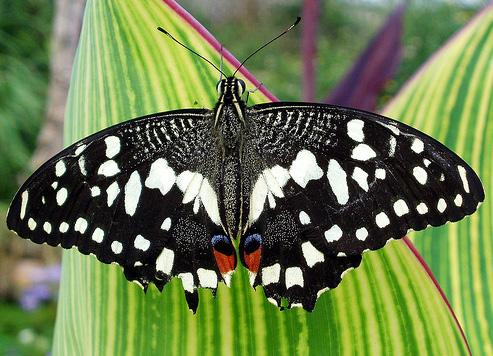
\includegraphics[width=0.4\textwidth]{Figures/butterfly.jpg}} \\
        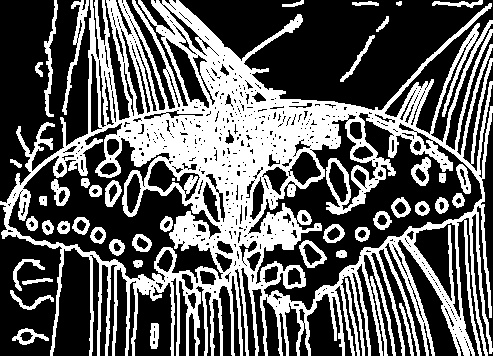
\includegraphics[width=0.4\textwidth]{Figures/butteredge.jpg} &
        
\includegraphics[width=0.4\textwidth]{Figures/butter.eps}
    \end{tabular}
    \caption[Conversion to Vector Graphics]{Conversion to Vector Graphics. While the vectorised image (bottom right) is clearly of the edge detection (bottom left), it utilises heavy approximation.}
    \label{fig:potrace}
    \end{center}
\end{figure}

When the documents were received by the server, they were converted back to OpenCV bitmaps using a custom interpreter built for the project. Both due to the approximation applied by Potrace and the custom interpreter not including all the necessary functions to accurately convert the vector files back to bitmaps, the final result loses much of its accuracy to the original image (Figure \ref{fig:potracecomp}). Due to the high edge accuracy requirements of producing a depth map from edge detected images, this method was discarded in favour of standard image compression. 

\begin{figure}[H]
    \begin{center}
    \begin{tabular}{ c c }
        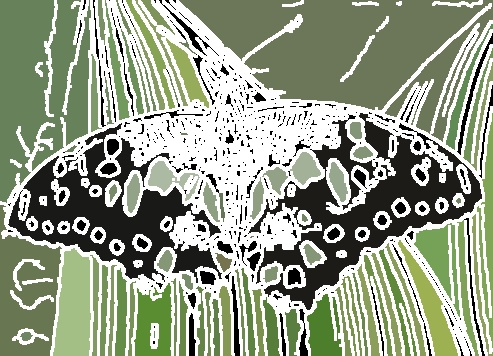
\includegraphics[width=0.4\textwidth]{Figures/buttercan.jpg} &
        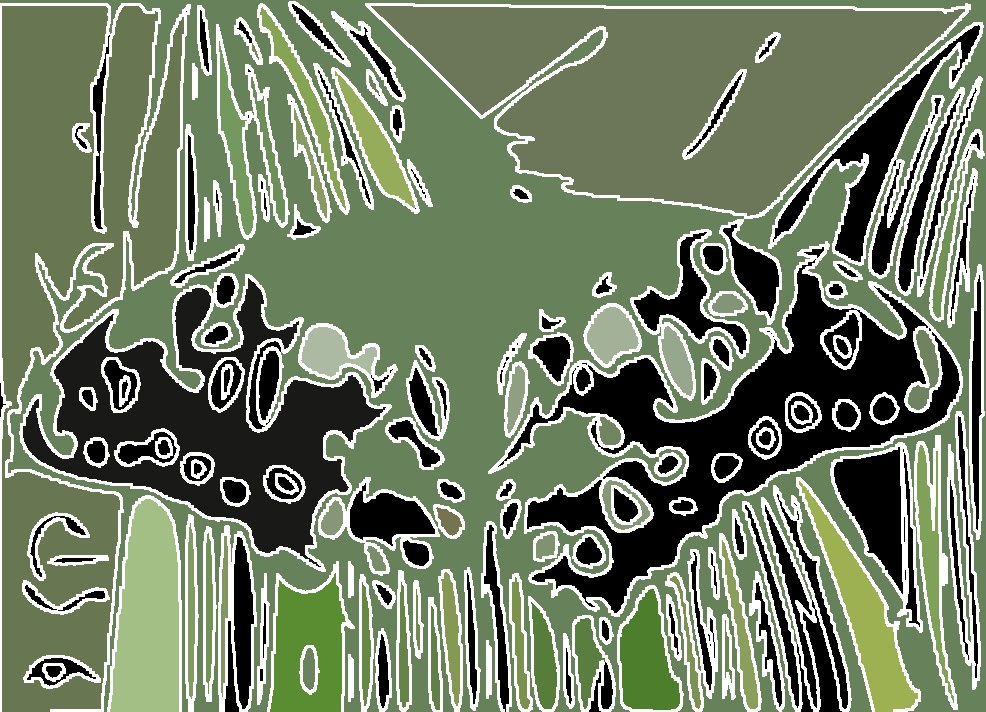
\includegraphics[width=0.4\textwidth]{Figures/butterred.jpg}
    \end{tabular}
    \caption[Comparison of Vector and Bitmap Accuracy]{Comparison of Vector and Bitmap Accuracy. Once the vector image has been converted back into a bitmap (right), it has lost much of its resemblance to the original image. A comparison to the image that results from transmitting compressed bitmaps (left) shows the sheer number of edges that have been either lost or combined together.}
    \label{fig:potracecomp}
    \end{center}
\end{figure}